\documentclass[%
    a0paper,%
    20pt,%
    portait,%
    margin=0mm,%
    innermargin=10mm,%
    blockverticalspace=10mm,%
    colspace=10mm,%
    subcolspace=5mm%
]{tikzposter}

\input{config.tex}

\addbibresource{ref.bib}

\author{T. Dehaeze, M. Magnin-Mattenet, C. Collette}
\date{2018-09-06}
\title{Sample Stabilization for Tomography Experiments in Presence of Large Plant Uncertainty}
\institute{}

\useblockstyle{customstyle}

\begin{document}

\maketitle[%
    roundedcorners=2,
    linewidth=2mm,
    innersep=10mm,
    titletotopverticalspace=10mm,
    titletoblockverticalspace=10mm]

\block[]{}{\textbf{Abstract}
A new low emittance lattice storage ring is under construction at the ESRF.
In this new instrument, an upgraded end station for ID31 beamline must allow to position the samples along \emph{complex trajectories with a nanometer precision}.
In order to reach these requirements, samples have to be mounted on high precision stages, combining a capability of large stroke, spin motion, and active rejection of disturbances.
However, the precision is limited by thermal expansion and various imperfections
that are not actively compensated. Our approach is to add a Nano Active Stabilization System (NASS) which is composed of a 6DoF Stewart platform and a 6 DoF metrology system.
A 3D model of the end station updated with experimental data is developed.
As the mass of the samples may vary by up to two orders of magnitudes, robust control strategies are required to address such plant uncertainty.
The proposed control strategy are presented and applied on the developed model by conducting time domain simulations of tomography experiment in presence of instrumentation noise and system uncertainty.

%%% Local Variables: ***
%%% mode:latex ***
%%% TeX-master: "2018 - Student Day.tex"  ***
%%% End: ***}

\begin{columns}
\column{0.5}
\block[]{Introduction}{Within the framework of the ESRF Phase II Upgrade Programme, a new state-of-the-art end station for the high-energy beamline ID31 is under development.
Research in many scientific areas such as material and life sciences are increasingly looking for instruments with higher spatial resolution.
The design of the new end station will enable many hard X-ray characterization techniques such as reflectivity, wide angle diffraction and diffraction tomography.
The need of great versatility induces many constrains on the end station such as combining \emph{large stroke} (\(\approx\SI{10}{\milli\metre}\)), \emph{high precision} (\(\approx\SI{10}{\nano\metre}\)) while accepting samples with mass ranging from \(\SI{1}{\kilo\gram}\) to \(\SI{50}{\kilo\gram}\).

Many positioning end stations have been developed with an increasing positioning precision \cite{martinez2016,DucotteMEDSI2016,ogurreck2013nanotomography}.

However, when nanometer precision is needed, thermal expansion and vibrations are becoming the main source of positioning error that cannot be compensated by encoders used for each stage.
Therefore, a direct metrology system is usually needed \cite{DucotteMEDSI2016}.

The aim of this study is to \emph{develop a short stroke Stewart platform that actively stabilize the sample position and compensate for all sources of perturbations and imperfection}.

\begin{tikzfigure}[Schematic of the Tomography Experiment]
\label{fig:exp_full_setup}
\centering
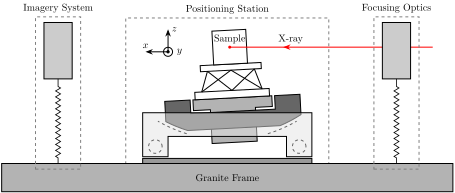
\includegraphics[width=0.95\linewidth]{./figs/exp_full_setup.pdf}


\end{tikzfigure}

%%% Local Variables: ***
%%% mode:latex ***
%%% TeX-master: "2018 - Student Day.tex"  ***
%%% End: ***}
\block[]{ID31 Sample Station}{\begin{tikzfigure}[CAD view of the ID31 end station]
\label{fig:assemblage}
\centering
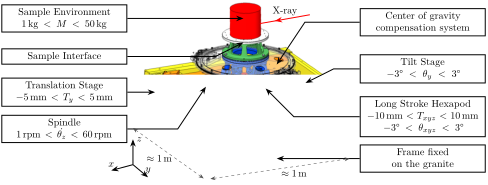
\includegraphics[width=\linewidth]{./figs/assemblage.pdf}


\end{tikzfigure}

\begin{minipage}[t]{0.49\linewidth}
  The ID31 Sample Station consists of multiple stacked stages
  (figs~\ref{fig:assemblage} and~\ref{fig:exp_setup}):



  \begin{itemize}
  \item \emph{translation stage}: travel range of \(T_y =
    \SI{\pm5}{\milli\metre}\). Permits to scan the sample through the X-ray.
  \item \emph{tilt stage}: rotates the sample around the \(y\) axis by
    \(\theta_y = \ang{\pm3}\). The rotation axis is aligned with the focusing
    point of the X-ray in order to allow experiments such as X-ray reflectivity.
  \item \emph{air bearing spindle}: rotate the sample around the vertical axis
    with an angular speed that varies from \(\dot{\theta_z} = \SI{1}{rpm}\) for
    light samples (\(M<\SI{1}{\kilo\gram}\)) to \(\dot{\theta_z} = \SI{60}{rpm}\)
    for heavy samples (\(M=\SI{50}{\kilo\gram}\)).
  \item \emph{long-stroke Stewart platform}: allows a fine positioning of the
    sample in all 6 degrees of freedom (DoF).
  \item \emph{gravity compensation system}: consists of two motorized mass that
    can be positioned around a circular guidance in order to perfectly aligned the
    center of mass with the spindle rotation axis.
  \item \emph{sample environment}: permits to study samples under wide range of
    condition: low (\(\SI{1.2}{\kelvin}\)) to high (\(\SI{2000}{\kelvin}\)) temperatures, high
    magnetic field (\(\SI{8}{\tesla}\)), etc.
  \end{itemize}
\end{minipage}\hfill
\begin{minipage}[t]{0.49\linewidth}
  \begin{tikzfigure}[Picture of the ID31 end station. (1) Granite, (2) Translation stage, (3) Tilt stage, (4) Long stroke hexapod, (5) Mass representing the sample environment. The spindle is hidden by the translation and tilt stages.]
  \label{fig:exp_setup}
  \centering
  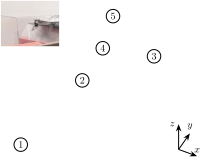
\includegraphics[width=\linewidth]{./figs/exp_setup.pdf}


  \end{tikzfigure}

  \begin{tikztable}[Specifications on the motions of the ID31 end station]
    \label{table:specifications}
    \centering
    \begin{tabular}{ccccc}
      \toprule
      & \(T_{xy}\) & \(T_z\) & \(\theta_y\) & \(\theta_z\)\\
      \midrule
      Repeatability & \(\SI{20}{\nano\metre}\) & \(\SI{10}{\nano\metre}\) & \(\SI{5}{\micro\radian}\) & \(\SI{2}{\micro\radian}\)\\
      MIM & \(\SI{3}{\nano\metre}\) & \(\SI{3}{\nano\metre}\) & \(\SI{2}{\micro\radian}\) & \(\SI{0.5}{\micro\radian}\)\\
      \bottomrule
    \end{tabular}
  \end{tikztable}
\end{minipage}\\

%%% Local Variables: ***
%%% mode:latex ***
%%% TeX-master: "2018 - Student Day.tex"  ***
%%% End: ***}

\column{0.5}
\block[]{Nano Active Stabilization System}{\begin{wrapfigure}[16]{r}{0.45\linewidth}
  \vspace{-2em}
  \begin{tikzfigure}[Schematic representation of the NASS added below the sample and the control architecture used]
  \label{fig:system_control}
  \centering
  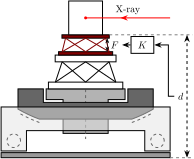
\includegraphics[width=0.9\linewidth]{./figs/system_control.pdf}


  \end{tikzfigure}
\end{wrapfigure}

\textbf{6 DoF Metrology System}
In order to achieve the positioning accuracy and stability requirements (shown on Table \ref{table:specifications}), a direct measurement of the relative position from the sample to the optical element is mandatory.
\emph{Laser interferometry} is chosen as it offers many advantages such as high resolution, high stability and large measurement range.

\vspace{1em}

\textbf{6 DoF Active Stabilization Stage}
In order to actively compensate the positioning error of the sample in all 6
DoF, a short stroke Stewart platform is added just below the sample as shown Figure~\ref{fig:system_control}.

By inverting the dynamics of the Stewart platform, it is possible to control independently the position of the mobile platform in all 6 DoF with respect to the fixed platform \cite{McInroy2000}.

\vspace{1em}

\textbf{Control Objective}
The control objective is to stabilize the position of the sample using the NASS actuators based on the 6DoF measurements provided by the metrology system.

Using this architecture, all the imperfections that cannot be compensated using the actual system (thermal drifts, guidance flexibilities, etc.) will be measured and compensated using a feedback control loop.

\vspace{1em}

\begin{minipage}[t]{0.63\linewidth}
  \textbf{Requirements For The NASS}
  The required stroke for the NASS should correspond to the maximum global
  positioning error of the end station without the NASS (\(\approx \SI{10}{\micro\metre}\) in translations).
  The repetability of the NASS is determined by the global specifications (Table \ref{table:specifications}).

  Other requirements such as stiffness and dynamical properties will be determined using the model presented below.
\end{minipage}
\begin{minipage}[t]{0.37\linewidth}
  \vspace{-1em}
  \begin{tikztable}[Rough estimation of the NASS specifications]
    \label{table:nass_specification}
    \centering
    \begin{tabular}{ccc}
      \toprule
      \textbf{Motion} & \textbf{Stroke} & \textbf{Repetability}\\
      \midrule
      \(T_{xyz}\) & \(\SI{\pm 10}{\micro\metre}\) & \(\SI{10}{\nano\metre}\)\\
      \(\theta_{xyz}\) & \(\SI{\pm 10}{\micro\radian}\) & \(\SI{1.7}{\micro\radian}\)\\
      \bottomrule
    \end{tabular}
  \end{tikztable}
\end{minipage}


% \textbf{Model Based Design}
% Such positioning system with multiple stages is highly coupled and presents many physical effects such as wobble that are difficult to model with a simple model based on measurements.
% Therefore, we have chosen to develop a 3D finite mass model. The software used is Simscape which is a toolbox for modeling multidomain physical systems within the Simulink environment.

% Each stage is represented as a 3D rigid body connected with the other stages by joints. Springs and dampers are added to take into account the finite stiffness of the mechanical guidance.
% Actuators and sensors dynamics are also included in the model.
% Finally, sources of perturbation and noise such as ground motion and sensor noise are also modeled.

% Thanks to the individual identification of each stage, stiffness and damping representing the flexibilities can be tuned properly.

% This model has numerous utility.
% First, it allows to conduct simulations of experiments such as tomography. That will help us to attest the performances of the system and compare various control architecture.
% Second, it permits to study the effect of the sample mass on the mechanical behavior of the system and verify the robustness properties of the controlled system.
% Finally, this model will be of great help for designing the NASS. Indeed, many parameters have to be properly chosen such as geometric configuration, leg stiffness, actuator type and rotational joints.

% In the following, the NASS is modeled as a Stewart platform with a cubic configuration, voice coil linear actuators and ideal rotational joints.

%%% Local Variables: ***
%%% mode:latex ***
%%% TeX-master: "2018 - Student Day.tex"  ***
%%% End: ***}
\block[]{Results}{% \textbf{Plant Identification}
% Various transfer functions of the system can be identified using the model.
% The most important one for control is \(G\) which is the transfer function from a force applied by the NASS to the measurement of the sample displacement. This represent the transfer function from \(F\) to \(d\) on Figure~\ref{fig:system_control}.

% \begin{minipage}{0.60\linewidth}
%   \begin{tikzfigure}[Transfer function from a force applied by the NASS to the sample displacement]
%   \label{fig:G_x_mass}
%   \centering
%   \includegraphics[height=12cm]{./figs/G_x_mass.pdf}


%   \end{tikzfigure}
% \end{minipage}\hfill
% \begin{minipage}{0.38\linewidth}
%   \begin{tikzfigure}[General control configuration]
%   \label{fig:general_conf_K}
%   \centering
%   \includegraphics[height=12cm]{./figs/general_conf_K.pdf}


%   \end{tikzfigure}
% \end{minipage}\\


% As the measurement and the force applied by the NASS are in 6DoF, \(G\) is a 6 by 6 transfer function.
% Figure~\ref{fig:G_x_mass} represents the bode diagram of the first element of \(G\) for 3 values of the sample mass.
% It shows that the sample mass has an important impact on the dynamic of the system and it confirms that we will have to be very cautious about the robustness of the controlled system.

\textbf{Control Configuration}
In order to control such a system, we choose to start with a simple centralized
feedback control as shown Figure~\ref{fig:general_conf_K}.
The controller takes the signal of the metrology system in 6DoF and generates
the forces applied by the NASS in 6DoF. It is therefore a 6 by 6 matrix.
\begin{minipage}{0.49\linewidth}
  \begin{tikzfigure}[Control configuration. \(P\) is the model of the end station, \(w\) the exogenous inputs, \(d\) the 6DoF measurement, \(F\) the 6DoF forces applied by the NASS and \(z\) the signals we want to minimize.]
  \label{fig:general_conf_K}
  \centering
  \includegraphics[height=13cm]{./figs/general_conf_K.pdf}


  \end{tikzfigure}
\end{minipage}\hfill
\begin{minipage}{0.49\linewidth}
  \begin{tikzfigure}[Positioning error of the sample during the simulation of a tomography experiment. The blue curve correspond with the ID31 without the NASS and the red curve with the NASS added. \(M=\SI{20}{\kilo\gram}\) and \(\dot{\theta_z} = \SI{30}{rpm}\).]
  \label{fig:exp_w_wo_nass_xy}
  \centering
  \includegraphics[height=13cm]{./figs/exp_w_wo_nass_xy.pdf}


  \end{tikzfigure}
\end{minipage}\\

\textbf{Control Synthesis}
We first choose to only have non-zero diagonal elements. Then, each diagonal
controller is tuned independently and has a lead-lag structure:
\begin{itemize}
\item An integral action is added at low frequency to have no static error
\item A lead is added near the crossover frequency to add some phase margin
\item A pole is further added in high frequency to reduce the effect of noise
\end{itemize}

\textbf{Tomography Experiment}
In order to test the performances obtained with the current controlled system, a simulation of a tomography experiment is conducted.
The rotation speed of the spindle is set to \(\dot{\theta_z} = 30rpm\), the mass of the sample is chosen to be \(M=\SI{20}{\kilo\gram}\), and ground motion is taken into account.

The result is shown Figure~\ref{fig:exp_w_wo_nass_xy}. The blue and the red curves represent the \(x-y\) motion of the sample for the positioning system respectively without the NASS and with the NASS.

The residual motion of the sample when using the NASS is less than \(\SI{50}{\nano\metre}\) in the \(xyz\) directions.

%%% Local Variables: ***
%%% mode:latex ***
%%% TeX-master: "2018 - Student Day.tex"  ***
%%% End: ***}
\block[]{Conclusion}{% \textbf{Conclusion}
A high precision and versatile positioning platform has been presented.
In order to obtain nanometer precision, a Stewart platform based stabilization system (the NASS) is proposed.
A 3D finite mass model has been developed to test such stabilization system. It has been showed that even with a simple control architecture, the parasitic motions of the sample can be reduced down to \(\SI{50}{\nano\metre}\).

These type of stabilization platform associated with a precise 6 DoF metrology system could be used for many other positioning systems.

To further improve the performance of the system, many control architecture could be developed such as a hybrid feedback-feedforward control or HAC-LAC feedback control. Moreover, to address the robustness issue, control techniques such as \(\mathcal{H}_\infty\) loop-shaping and \(\mu\)-synthesis would be of great help.

%%% Local Variables:
%%% mode: latex
%%% TeX-master: "2018 - Student Day"
%%% End:
}
\end{columns}

\block[]{}{\textbf{Reference}
\printbibliography[heading=none]
% \vspace{-1em}

\textbf{Acknowledgments}
This research was made possible by a grant from the ESRF.
We thank the following people for their support, without whose help this work would never have been possible: V. Honkimaki, A. Jublan, L. Ducotte, C. Carole, M. Brendike and M. Lessourd and the whole team of the Precision Mechatronic Laboratory.

%%% Local Variables: ***
%%% mode:latex ***
%%% TeX-master: "2018 - Student Day.tex"  ***
%%% End: ***}
% \block[]{}{\input{acknoledgment.tex}}

\end{document}
\section{ACKNOWLEDGMENTS}
\label{sec:org59f58a9}
This research was made possible by a grant from the ESRF.
We thank the following people for their support, without whose help this work would never have been possible: V. Honkimaki, A. Jublan, L. Ducotte, C. Carole, M. Brendike and M. Lessourd and the whole team of the Precision Mechatronic Laboratory.